\documentclass[a4paper]{article}

% font stuff
%\usepackage{mathptmx}
\usepackage{fouriernc}
\usepackage[T1]{fontenc}

\usepackage{amsmath}
\usepackage{amssymb}
\usepackage{amsthm}
\usepackage[retainorgcmds]{IEEEtrantools}
%\usepackage[square]{natbib}

% needs debian package texlive-math-extra
\usepackage{stmaryrd} % for \llbracket, \rrbracket (scott brackets)

\usepackage{tikz}
\usetikzlibrary{positioning}
\usetikzlibrary{matrix}

\newcommand{\below}{\sqsubseteq}
\newcommand{\arr}{\rightarrow}
\newcommand{\todo}[1]{\bigskip \noindent \emph{todo: #1}}
%\newcommand{\todo}[1]{}
\newcommand{\semantics}[1]{\llbracket #1 \rrbracket}
\newcommand{\lub}{\bigsqcup}
\newcommand{\set}[1]{\{\,#1\,\}}

% They all use the same counter, reset at section boundaries
% This gives a running number:
% Section 1
%   Theorem 1.1
%   Definition 1.2
%   Lemma 1.3
% Section 2
%   Definition 2.1
%   Lemma 2.2
%   ...
\newtheorem{definition}{Definition}[section]
\newtheorem{theorem}[definition]{Theorem}
\newtheorem{proposition}[definition]{Proposition}
\newtheorem{lemma}[definition]{Lemma}

\begin{document}

\title{Thesis}
\author{Markus Klinik}
\maketitle

\begin{abstract}

Abstract

\end{abstract}

\section{Introduction}

Introduction

\section{Domain Theory}


\begin{definition}

Let $D$ be a poset, $S \subseteq D$. The \emph{least upper bound} (``lub'') of $S$
is an element $x \in D$ such that:

\begin{equation} \label{eqnLub1}
\forall y \in S \ldotp y \below x
\end{equation}
\begin{equation} \label{eqnLub2}
\forall z \in D \ldotp (\forall y \in S \ldotp y \below z) \implies x \below z
\end{equation}

The lub of S, if it exists, is denoted interchangeably by
\begin{IEEEeqnarray*}{rCl}
\lub S = \lub_{x \in S} x = \lub \set{x \mid x \in S}
\end{IEEEeqnarray*}

\end{definition}


Line (\ref{eqnLub1}) states that the lub is above all elements: it is an upper
bound, and (\ref{eqnLub2}) states that the lub is below any other upper bound:
it is the least such. If a lub exists, it is unique. It is therefore justified
to call it \emph{the} lub.


\begin{definition}

A \emph{chain} in a poset is a linearly ordered subset.

\end{definition}


\begin{definition}

Let $D$ be a poset. A set $S \subseteq D$ is \emph{directed} iff every finite
$P \subseteq S$ has an upper bound in $S$.

\end{definition}


In literature on domain theory and semantics of programming languages, one
encounters three different definitions of complete partial orders.  There is
chain-completeness: \cite{Moschovakis1994}, directed-completeness:
\cite{DaveyPriestly1990}, \cite{Gunter1992}, and $\omega$-sequence-completeness:
\cite{Allison1986}, \cite{Winskel1993}, \cite{BarrWells1990}. Abramsky and Jung
\cite{Abramsky1994} have a short discussion on the equivalence of these
definitions, but refer to further literature for proofs. The proof given here
occurs as an exercise in Davey and Priestly \cite{DaveyPriestly1990}.


\begin{definition} \label{defCpoDirectedComplete}

(directed-complete) A \emph{cpo} is a partial order where every directed set has
a least upper bound.

\end{definition}


\begin{definition} \label{defCpoChainComplete}

(chain-complete) A \emph{cpo} is a partial order where every chain has a least
upper bound.

\end{definition}


\begin{definition} \label{defCpoOmegaSequenceComplete}

($\omega$-sequence-complete) A \emph{cpo} is a partial order where every
non-decreasing sequence of elements $x_0 \below x_1 \below x_2 \below \ldots $
has a least upper bound.

\end{definition}


\begin{proposition}

The three definitions of cpos are equivalent.

\end{proposition}


We give a round-robin proof, of which two implications are fairly simple. The
third implication is a bit more involved, and requires the axiom of choice. We
give a proof for the countable case here because it is illustrative, and refer
to the literature for the uncountable case.


\begin{proof}

$\ref{defCpoDirectedComplete} \implies \ref{defCpoChainComplete}$: Every chain
is directed.

$\ref{defCpoChainComplete} \implies \ref{defCpoOmegaSequenceComplete}$:
The image of a non-decreasing $\omega$-sequence is a chain.

$\ref{defCpoOmegaSequenceComplete} \implies \ref{defCpoDirectedComplete}$: Let
$D$ be an $\omega$-sequence-complete cpo as in definition
\ref{defCpoOmegaSequenceComplete}, let $S = \set{x_0, x_1, x_2, \ldots}
\subseteq D$ be countable and directed. For each finite $F \subseteq S$, let
$u(F)$ be some upper bound of $F$ in $S$.  Construct a sequence of sets $P_n
\subseteq S$ as follows,
\begin{IEEEeqnarray*}{rCl}
P_0 & = & \set{x_0} \\
P_{n+1} & = & P_n \cup \set{u(P_n \cup y_n), y_n}
\end{IEEEeqnarray*}

where $y_n$ is the $x_i \in S\backslash P_n$ with the smallest possible $i$.

Every $P_n$ is directed: $P_0$ certainly is, and any finite subset of $P_{n+1}$
has $u(P_n \cup y_n) \in P_{n+1}$ as upper bound.  As every $P_n$ is finite and
directed, taking its lub is justified.

Consider the $\omega$-sequence $Q$ = $\set{\lub P_n}_{n \in \mathbb{N}}$. For
all $n$, we have $P_n \subseteq P_{n+1}$ and thus $\lub P_n \below \lub
P_{n+1}$, so $Q$ is non-decreasing, and therefore has a lub $z$.  Each $x \in S$
eventually occurs in some $P_n$, and we have $x \below \lub P_n \below z$, so
$z$ is an upper bound of $S$. Any upper bound $z'$ of $S$ is also an upper bound
of $Q$, and therefore $z \below z'$, i.e. $z$ is the lub of $S$.

\end{proof}


The complication in the third implication comes from the fact that a directed
set doesn't need to be linearly ordered. Every directed set does however contain
a chain which threads through the whole set, eventually rising above all
elements. The lub of the chain is then the lub of the directed set.


\subsection{The Category Cppo}


\begin{definition}

A cpo $D$ is \emph{pointed} iff it has a bottom element $\bot$ which
satisfies $\forall d \in D \ldotp \bot \below d$.

\end{definition}

\begin{definition}

Let $C$, $D$ be partial orders. A function $f : C \arr D$ is \emph{monotone} iff
it is order preserving, that is for all $x, y \in C$,
\begin{IEEEeqnarray*}{rCl}
  x \below y \implies f(x) \below f(y)
\end{IEEEeqnarray*}

\end{definition}

\begin{definition}

Let $C$, $D$ be cpos. A function $f : C \arr D$ is \emph{continuous} iff it
is monotone and preserves lubs, that is for all chains $P \subseteq C$,
\begin{IEEEeqnarray*}{rCl}
  f(\lub_{x \in P} x) = \lub_{x \in P} f(x)
\end{IEEEeqnarray*}

\end{definition}

Note that if a function preserves lubs, it is monotone,
\begin{IEEEeqnarray*}{rCl}
  x \below y \implies
  y = \lub \set{x, y} \implies
  f(y) = f(\lub \set{x, y}) = \lub \set{f(x), f(y)} \implies
  f(x) \below f(y)
\end{IEEEeqnarray*}

but in a proof of continuity of a function $f$, we usually need to prove
monotonicity as a first step, so that for a chain $P$, $\set{f(x) \mid x \in P}$
is again a chain. This motivates the inclusion of
monotonicity in the definition of continuity.


\begin{lemma}

The identity function is continuous.

\end{lemma}

\begin{proof}

Let $P \in C$ be a chain. Then
\begin{equation*}
id(\lub P) = \lub P = \lub_{x \in P} id(x)
\end{equation*}

\end{proof}


\begin{lemma}

Composition of two continuous functions is continuous.

\end{lemma}

\begin{proof}

Let $f : C \arr D$, $g : D \arr E$ be continuous. Let $P \subseteq C$ be a
chain. Then
\begin{IEEEeqnarray*}{rCl}
(g \circ f)(\lub P) & = & g(f(\lub_{x \in P} x)) \\
  & = & g( \lub_{x \in P} f(x) ) \\
  & = & \lub_{x \in P} g(f(x)) \\
  & = & \lub_{x \in P} (g \circ f)(x)
\end{IEEEeqnarray*}

\end{proof}


\begin{proposition}

The complete pointed posets, together with continuous functions between them form
a category.  This category is called Cppo.

\end{proposition}


\begin{definition}

A category has the \emph{fixpoint property} iff for all objects $A$ and arrows
$f : A \arr A$ there exists an arrow $Y(f) : 1 \arr A$ such that $Y(f) = f
\circ Y(f)$.

\end{definition}


\begin{theorem}

Cppo has the fixpoint property.

\end{theorem}

\begin{proof}

Let $D$ be a cppo, $f : D \arr D$ a continuous function. Whe have to show that
there exists an element $x \in D$ such that $x = f(x)$. Consider the set
\begin{equation*}
F = \set{f^n(\bot) \mid n \in \mathbb{N}}.
\end{equation*}
This set is a chain, because for $n = 0$
we have $f^0(\bot) = \bot \below f(\bot)$. Now assume that $f^n(\bot) \below
f^{n+1}(\bot)$. Then $f(f^n(\bot)) \below f(f^{n+1}(\bot))$, so $f^{n+1}(\bot)
\below f^{n+2}(\bot)$. Because $F$ is a chain and $D$ a cppo, $F$ has a lub $x =
\lub F$.  We calculate:
\begin{IEEEeqnarray*}{rCl}
f(x) & = & f(\lub F) \\
     & = & \lub f(F) \\
     & = & \lub \set{ f(f^n(\bot)) \mid n \in \mathbb{N} } \\
     & = & \lub \set{ f^{n+1}(\bot) \mid n \in \mathbb{N} } \\
     & = & \lub \set{ f^n(\bot) \mid n \in \mathbb{N} } \\
     & = & \lub F = x
\end{IEEEeqnarray*}

\end{proof}

This is the well-known fixpoint theorem, which is sometimes attributed to
Tarski, sometimes to Kleene, but while they both knew the result, its actual
origin seems to be lost in time \cite{Lassez1982}. The formulation given here
is due to Huwig \cite{Huwig1990}.





\section{Junkyard}

\begin{figure}[ht]
\begin{center}
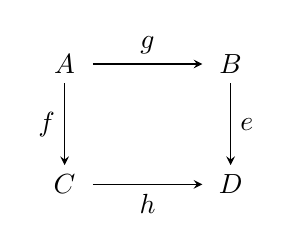
\begin{tikzpicture}
\matrix (m) [matrix of math nodes,row sep=3em,column sep=4em,minimum width=2em]
  {
     A & B \\
     C & D \\
  };
  \path[-stealth]
    (m-1-1) edge node [left] {$f$} (m-2-1)
            edge node [above] {$g$} (m-1-2)
    (m-2-1.east|-m-2-2) edge node [below] {$h$} (m-2-2)
    (m-1-2) edge node [right] {$e$} (m-2-2);
\end{tikzpicture}
\end{center}
\caption{Example of a comutative diagram}
\end{figure}

\begin{figure}
\begin{center}
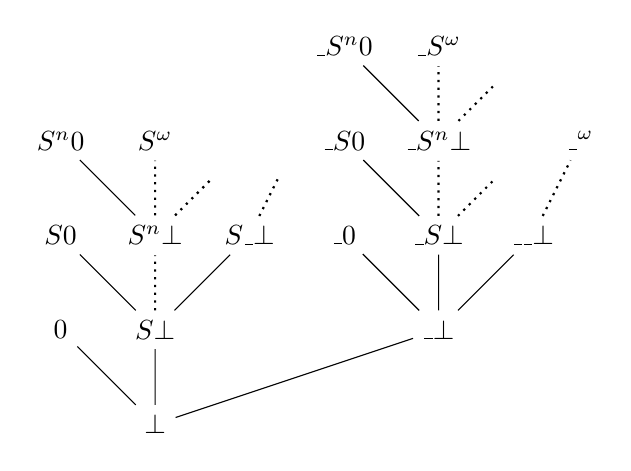
\begin{tikzpicture}
 [ grow'=up
 , scale=1.2
 , level distance=1cm
 , level 1/.style={sibling distance=3cm}
 , level 2/.style={sibling distance=1cm}
 , normal/.style={thin, solid}
 , skipping/.style={thick, dotted}
 , and so on/.style={thick, dotted, sibling distance=0.6cm, level distance=0.6cm}
 ]
  \node {$\bot$}
    child [sibling distance=1cm] { node {$0$} }
    child
    {
      node {$S\bot$}
      child { node {$S0$} }
      child [skipping]
      {
        %node {$SS\bot$}
        %child { node {$SS0$} }
        %child [skipping]
        %{
          node {$S^n\bot$}
          child [normal] { node {$S^n0$} }
          child [skipping] { node {$S^\omega$} }
          child [and so on] {}
        %}
        %child [and so on] {}
      }
      child
      {
        node {$S\_\bot$}
        child [missing] {}
        child [and so on] {}
      }
    }
    child
    {
      node {$\_ \bot$}
      child { node {$\_0$} }
      child
      {
        node {$\_S\bot$}
        child { node {$\_S0$} }
        child [skipping]
        {
          node {$\_S^n\bot$}
          child [normal] { node {$\_S^n0$} }
          child { node {$\_S^\omega$} }
          child [and so on] {}
        }
        child [and so on] {}
      }
      child
      {
        node {$\_\_\bot$}
        child [missing] {}
        %child [missing] {}
        child [skipping] { node {$\_^\omega$} }
      }
    }
  ;
\end{tikzpicture}
\end{center}
\caption{The domain $(Z, \sqsubseteq)$.}
\label{figDomainOfNuF}
\end{figure}

\begin{figure}
\begin{center}
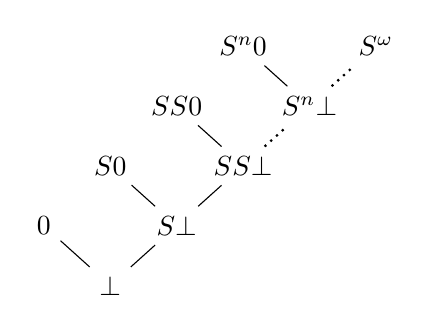
\begin{tikzpicture}[scale=1.2]
  \node {$\bot$} [grow'=up, sibling distance=4.0em, level distance=1.8em]
    child { node {$0$} }
    child
    {
      node {$S\bot$}
      child { node {$S0$} }
      child
      {
        node {$SS\bot$}
        child { node {$SS0$} }
        child [thick, dotted]
        {
          node {$S^n\bot$}
          child [thin, solid] { node {$S^n0$} }
          child { node {$S^\omega$} }
        }
      }
    }
  ;
\end{tikzpicture}
\end{center}
\caption{The domain of $L$, the lazy natural numbers.}
\label{figDomainOfLazyNaturals}
\end{figure}


\section{Further directions}

Left, left, right.

\section{Bibliographic notes}

This work is based on chapter 7 of the PhD thesis of Venanzio Capretta
\cite{Capretta2002}, where coinductive natural numbers are discussed.  Some
treatment of lazy natural numbers can be found in \cite{Escardo1993}.

A short introduction to dentotational semantics can be found in
\cite{Allison1986}, while \cite{Gunter1992} is a more comprehensive treatment of
that topic.  A view on domain theory and denotational semantics from the
perspective of category theory can be found in \cite{Pierce1991},
\cite{Bird1997}, \cite{Mitchell1996} and \cite{BarrWells1990}.


\bibliographystyle{plain}
\bibliography{computer_science}
\end{document}

% vim: textwidth=80
